
%\documentclass[10pt,notitlepage]{article}
%\nonstopmode  % to allow pdflatex to compile even if errors are raised (e.g. missing figures)


\documentclass[10pt]{beamer}
\nonstopmode  
\pagenumbering{arabic}
\usepackage{fancyhdr}
\usepackage{lastpage}
 
% Better and richer math environment
\usepackage{amsmath}

% EPS and PDF figures
\usepackage{graphicx}

% EPS and PDF figures
%\usepackage[nomarkers,figuresonly]{endfloat}


\usepackage{color}

\usepackage{beamerthemesplit}
\usepackage{graphicx} 

\usepackage{amssymb}
\usepackage{bm}
% \graphicspath{{./figures/}} % save all figures in the same directory
\usepackage{color} 
\usepackage{hyperref}
\usepackage{parskip}

\usepackage{enumerate}
%\pagestyle{empty}
\newcommand{\mysection}[1]{\section{{\normalsize {#1}}}}
\newcommand{\sub}[1]{\subsection{{\normalsize {#1}}}}
\newcommand{\subsub}[1]{\medskip \noindent {\bf {#1}}}

\usepackage{ifthen} 
\newboolean{includethis} 
\setboolean{includethis}{false} 
\newcommand{\given}{\mid}
\newcommand{\me}{\mathrm{e}} % use for base of the natural logarithm
\newcommand{\md}{\mathrm{d}} % use for base of the natural logarithm
\newcommand{\mean}{\mathrm{E}}
\newcommand{\Normal}{\mathcal{N}}
\newcommand{\argmax}{\operatornamewithlimits{argmax}}
\newcommand{\like}{\mathcal{L}}

\title{Modeling Posterior Effects: A Continuous Journey ....}
\author{Sarah Urbut}
\date{\today}
\begin{document}

\frame{\titlepage}



\frame{
\frametitle {Motivation}
\begin{itemize}
\item Variation in gene expression is an important mechanism underlying susceptibility to complex disease. 
\item However, most studies to date have been conducted in a single immortalized peripheral cell type or single tissue framework 
\item The solution! GTEx!	 by 2016: 900 post-mortem donors, with approximately 30 tissues collected from each donor
\item  Our mission: {\it jointly analyze data on all tissues} to maximize power, and to identify and quantify the variability in effect sizes.
\end{itemize}
}


\frame{
\frametitle {Specific Aims}
\begin{itemize}
\item  Develop statistical methods for estimating the effect size of QTLs in large numbers of diverse cell-types and tissues, thereby mapping QTLs.
\item Compare among methods of estimation.
\item Apply to GTEx Data

\end{itemize}
}



\frame{
\frametitle {Aim 1}
%\begin{itemize}
%\item
{\textbf {Develop methods of estimating the posterior effect size across multiple subgroups, thereby mapping eQTLs }}
\begin{itemize}
\item Combine information across tissues% to fully acknowledge the multi-tissue nature of a SNP
\item Report an effect size %rather than simply binary outcome to compare among SNPs called active within a tissue or among tissues
\item Capture distinct variation in effect sizes within and between subgroups: 'patterns of sharing' %better than restricting effects to simply 'shared' or 'unshared' between subgroups. 
%
\end{itemize}
}

\frame{
\frametitle{The Setting}
\begin{itemize}
\item{How do we quantify the effect of a particular SNP on gene expression among tissues?}
\item{Approach 1: The Isolationist Approach}
\end{itemize}
 \begin{figure}
\includegraphics[width=8cm]{Isolation.pdf}
\label{fig:Isolation}
\end{figure}
}




\frame{
\frametitle{The Setting}
\begin{itemize}
\item{How do we quantify the effect of a particular SNP on gene expression among tissues?}
\item{Approach 2: The Joint Committee Approach}
\itemRecognize the multivariate nature of this activity
\item Many different patterns of sharing of effects among tissues.
\item But how do we learn about the nature and frequency?
\end{itemize}
 \begin{figure}
\includegraphics[width=6cm]{joint.pdf}
\label{fig:Isolation}
\end{figure}
}



\frame{
\frametitle{Considering ALL the evidence!}
\begin{itemize}
%\item{\bf Jointly model the Posterior Effect Size $\bm{b}_{j}$ of gene-SNP pair $j$}
%\item Observe standardized multivariate effect size $\hat{\bm{b}}_{j}$
%\item Descend from true effect size  $\bm{b}_{j}$
\item Each eQTL may follow a particular pattern of activity %such that groups 
\item Within these groups, the tissues exhibit characteristic patterns of sharing of effects %, which can be 
 \begin{figure}
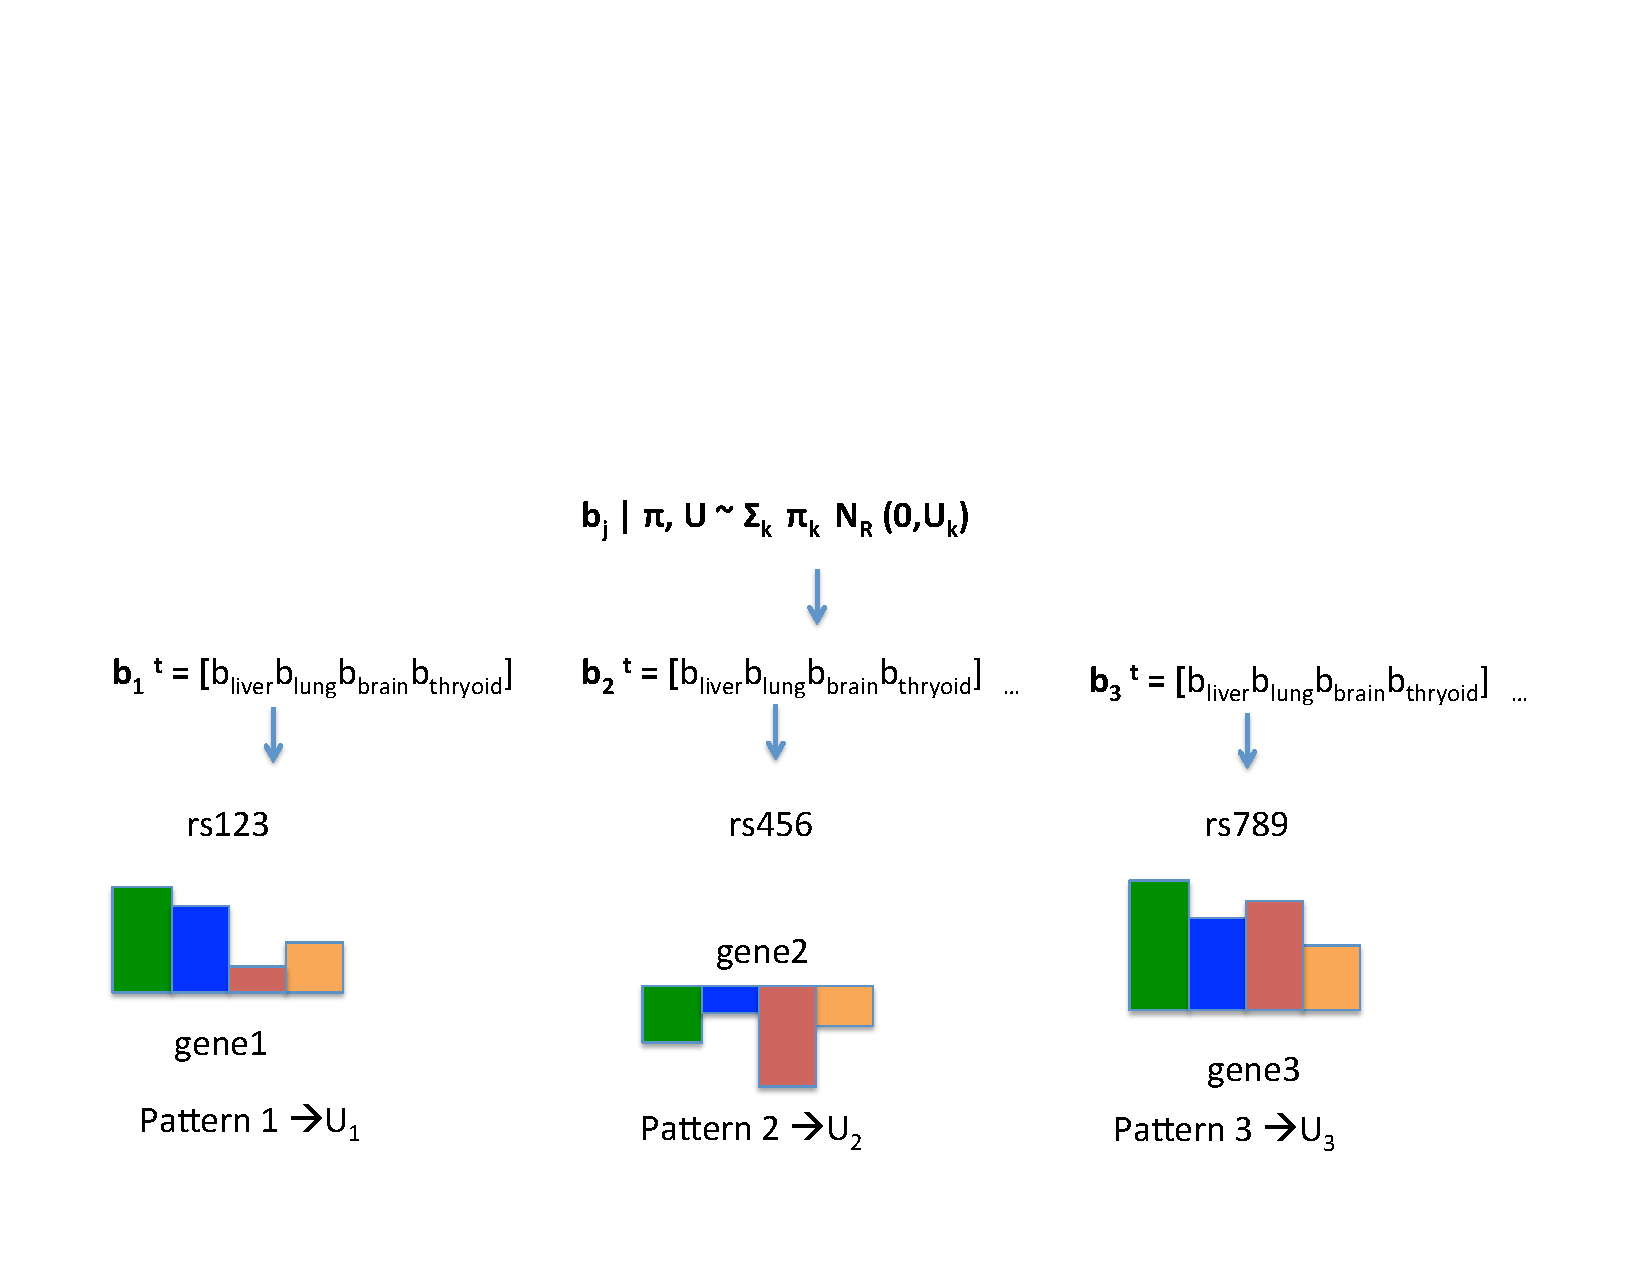
\includegraphics[width=6cm]{hm.pdf}
\end{figure}
\item Captured by considering the covariance structure of the genetic effects among tissues. 
%\item This lends itself to a mixture model, in which  we assume all the gene-snp pairs are generated from a mixture of a finite number of Gaussian distributions with unknown parameters. the multivariate nature of this activity, within a particular 'pattern of sharing' some tissues may be more active than others, but not completely on or off. Previous work from our lab considered only the idea that the covariance between two tissues was the same across tissues thought to contain a QTL in a given pattern, or 'configuration',  and thus failed to incorporate the much richer covariance structure between tissues. The primary novelty of this proposal is {\it to estimate this multivariate posterior distribution on the effect size in a data-sensitive way} - i.e., using the mixture model to capture information about the covariance structure among subgroups (here, tissues). 
\item Natural mixture model: Each component of the mixture is defined by the prior covariance matrix $U_{k}$ from which the vector of standardized effect sizes of this class is thought to be drawn. 
\item Learn relative frequencies from the data
\end{itemize}%\item component-specific covariance matrix then represents the variance of the effect size within and between tissues. 
}




\frame{
\frametitle{So what are the Prior Covariance Matrices $U_ks$ specifiying?}
Suppose we have just two tissues 

 \begin{figure}
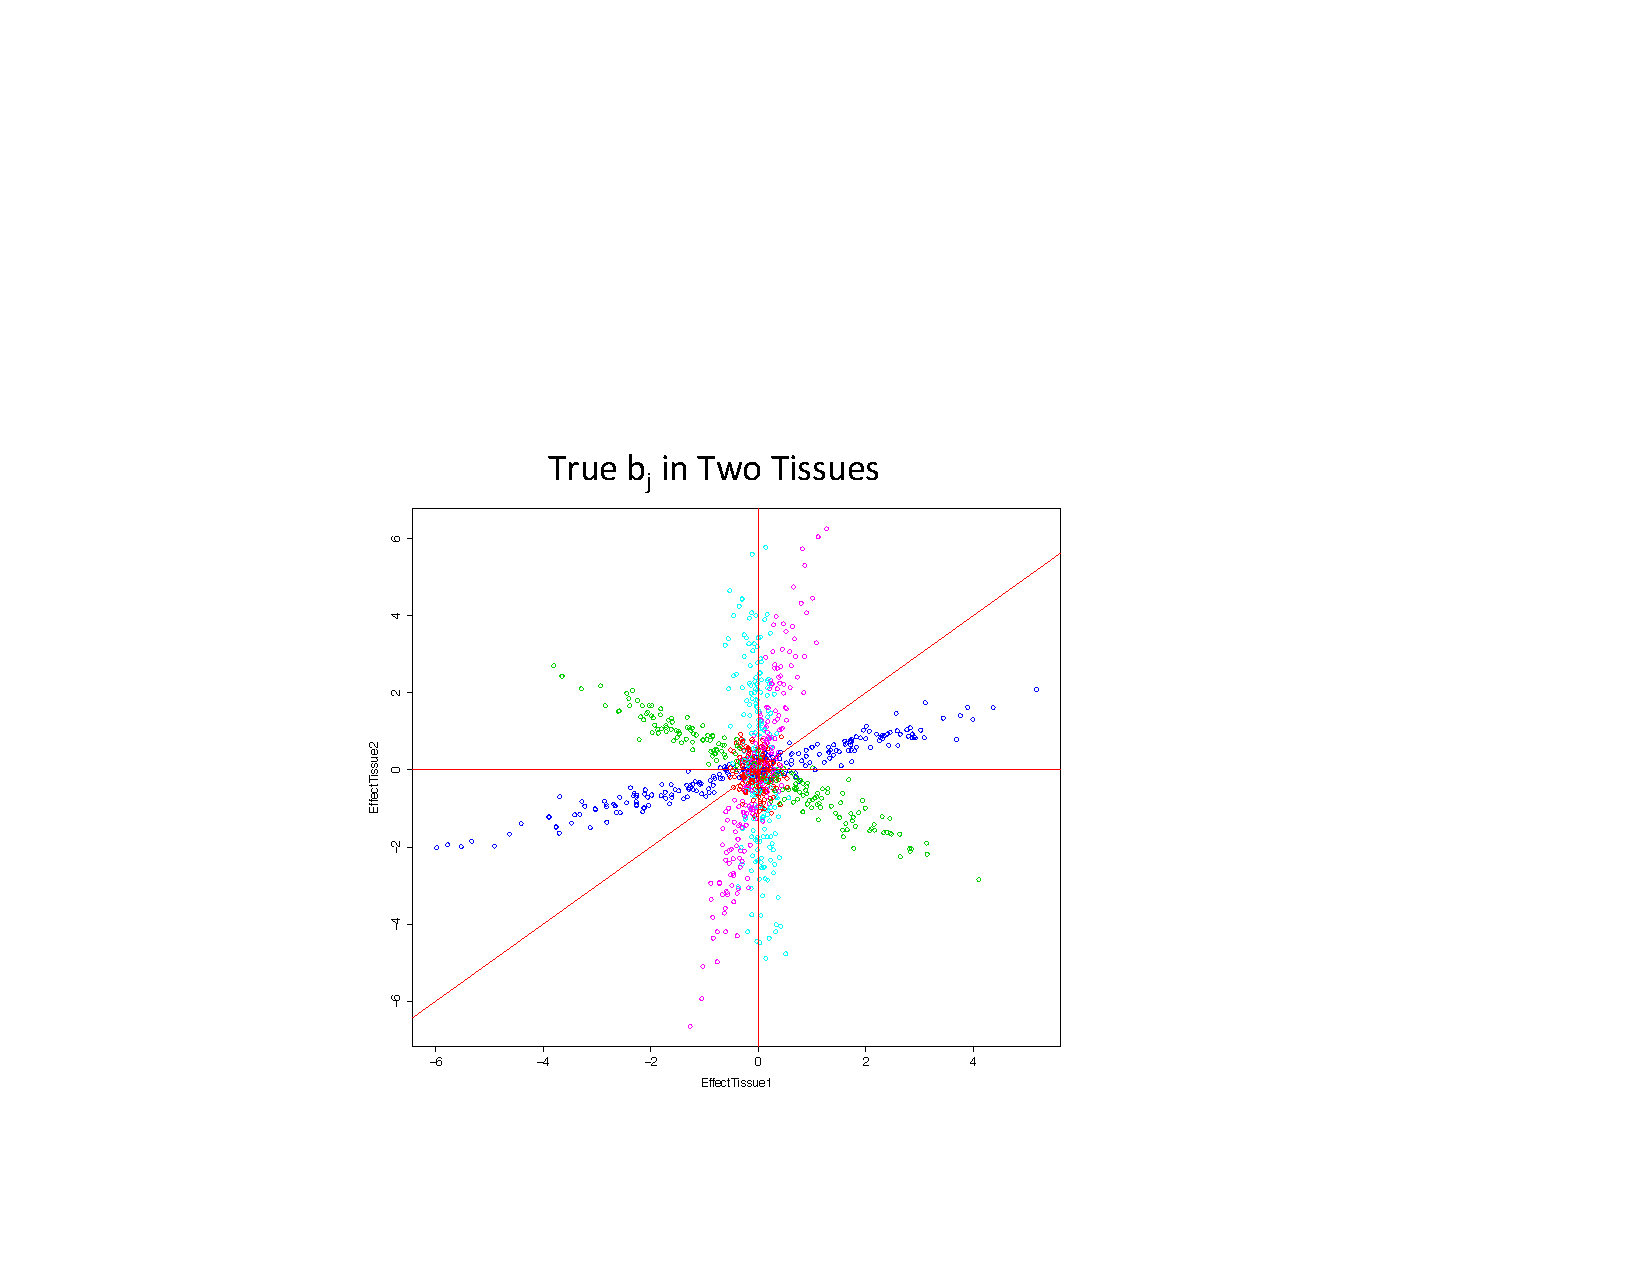
\includegraphics[width=5cm]{snptypes}
\end{figure}
\begin{itemize}
\item Direction defined by relative ratio in effect size between tissues, specified in prior covariance of $\bm{b}$
\end{itemize}

Generative $U_{k}$ for \textcolor{blue}{SNPs} 
\begin{pmatrix}
   Var(b_{1}) = \textcolor{blue} {2.0}  &  Cov(b_{1},b_{2})=0.56 \\
    Cov(b_{2},b_{1})=0.56 & Var (b_{2})=\textcolor{blue}{0.20}
 \end{pmatrix}
\item Additional novelty: Ratio between tissues is flexible (not simply shared or tissue-specific) and data sensitive (stay-tuned)

}

\frame{
\frametitle{Why care about the effect size?}

\begin{itemize}

\item Comparisons among tissues in which the QTL is called active, and among gene-snp pairs with a similar degree of activity in a given tissue. 
\item The addition of the quantitative comparison captures the continuous nature of biological phenomenon. %Estimating the distribution of multivariate effect sizes seems like a natural addition. The estimation procedure is non-trivial, and previous work by our lab (\cite{flutre_statistical_2013,wen_bayesian_2014}) applied a multivariate mixture model to estimate heterogeneity of effects among conditions.
\item How confident are we in the sign of the effect?
\item Acknowledge the many patterns of sharing present in the data, wide array of prior covariance matrices allows our gene-snp pair to find it`s true pattern of sharing


\end{itemize}
}


\frame{
  \frametitle{\it Mixture Prior}
For a given gene-snp pair, $\bm{b}$ represents the $R$ vector of unknown standardized effect. We model the prior distribution from which $\bm{b}$ is drawn as a mixture of multivariate {\it Normals}.
 
 \begin{equation}
  \label{prior_b_mixt_grid}
  \bm{b} | \bm{\pi},\bf{U} \sim \sum_{k,l} \pi_{k,l} \;{\it N}_R(\bm{0}, \omega_l U_{k})
\end{equation}

\begin{itemize}  
\item Choice of $U_k$ determines the direction, while $\omega_l$ determines the 'stretch' or 'tails' of each distribution
%\item `stretch factor' $\omega_{1\cdots L}$. 
\item $\pi_{k,l}$ to represent the (unknown) prior weight on prior covariance matrix $U_{k,l}$ %which represents a direction and stretch along this vector
\item  Use the EM algorithm to estimate the optimal combination of weights: How often does this particular pattern of sharing  occur in the data?
%\item Given a direction, may have different proportions of large and small effects
%\item The novelty of our approach is in modeling $\bm{b}_{j}$ as a mixture of multivariate {\it Normals}
\end{itemize} %where each component of the mixture is defined by its data-sensitive estimate of the prior covariance matrix $U_{k,l}$. We allow the latent variable $z_{j}$ to indicate which combination of covariance matrix and stretch factor we are considering,  $z_{j}$ can take on $KxL$ values $z_{j}$ = $[1,1] \cdots[k,l]$ .
}






\frame{
  \frametitle{\it For a given gene-snp pair: Likelihood for $\bm{b}$}

%By maximum likelihood in each tissue separately, we can easily obtain the estimates of the standardized genotype effect sizes, $\hat{\bm{b}}_{j}$, and their squared standard errors recorded on the diagonal of an $R \times R$ matrix noted $\hat{V}_{j} = \Var(\hat{\bm{b}}_{j})$. We assume that the matrix of standard errors of $\hat{\bm{b}}_{j}$, $V_{j}$ as approximated by $\hat{V_{j}}$ is diagonal and  that $\hat{V}_{j}$ is an accurate point estimate for the standard error and that these standard errors are independent between tissues.

%If we now view $\hat{\bm{b}}_{j}$ and $\hat{V}_{j}$ as \emph{observations} (i.e. known), we can write a new ``likelihood'' (using only the sufficient statistics) where we employ the use of bold typeset to indicate vector notation:

\begin{itemize}
\item ${\hat{\bm{b}}}$ : R x 1 vector of standardized maximum likelihood estimates of effect sizes 
\item $\hat{V} \approx Var(\hat{\bm{b}})$: RxR diagonal `accurate' approximation of standardized standard error of ${\hat{\bm{b}}}$.
%\item For each component, marginal likelihood: ${\it{N_R}(\hat{\bf{b}}; \bm{0}, U_{k} + \hat{V})}$
\item $\hat{\bm{b}}$ and $\hat{V}$ as \emph{observations} (i.e. known)
\end{itemize} 

For a given gene-snp pair, the Likelihood on $\bm{b}$: 
\begin{equation}
  \label{new_lik}
  \hat{\bm{b}} | \bm{b} \sim {\it N}_R(\bm{b}, \hat{V})
\end{equation}

}



\frame{
\frametitle{For a given gene-snp pair: Posterior on $\bm{b}$}
We know that for a single multivariate {\it Normal}  the posterior on  $\bm{b} | U_0$ is  simply: 
\[
\bm{b} | \hat{\bm{b}} \sim {\it N}_R(\bm{\mu}_{1}, U_{1})
\]
where:
\begin{itemize}
\item $\bm{\mu}_{1} = U_{1} (\hat{V}^{-1} \hat{\bm{b}})$;
\item $U_{1} = (U_{0}^{-1} + \hat{V}^{-1})^{-1}$.
\end{itemize}
}
%
%\frame{
%\frametitle{Really Not that Complicated}
%This leads us to a corresponding posterior that is also a mixture of multivariate {\it Normals} as this prior is conjugate to likelihood.
%


\frame{
\frametitle{For a given gene-snp pair: Posterior on $\bm{b}$}

\begin{itemize}
\item  Normal prior+ Normal likelihood = Normal posterior
\item  Mix normal prior + normal likelihood = Mix normal posterior
\end{itemize}

\begin{equation}
\begin{aligned}
  \label{eq:mixpost}
p(\bm{b}_ | \hat{\bm{b}}, \hat{V}, \hat{\bm{\pi}} )
&= \sum_{k=1,l=1}^{K,L} \sim {\it N}_R(\bm{\mu}_{1kl}, U_{1kl})%p(\bm{b}_{j} | \hat{\bm{b}}_{j}, \hat{V}_{j}, z_{j}=k,l) 
p(z=k,l | \hat{\bm{b}}, \hat{V}, \hat{\bm{\pi} }),%v_{j}=1)
 \\
&= \sum_{k=1,l=1}^{K,L} \sim {\it N}_R(\bm{\mu}_{1kl}, U_{1kl})%,v_{j}=1) 
\tilde \pi_{k,l}

\end{aligned}
\end{equation}

\begin{itemize}
\item $\tilde \pi_{k,l} = P(Component|Data) \propto  P(Data|Comp.) \times P(Comp.)$ 
Combine hierarchical and snp-specific information
\item  Allows pair to find its true match!
\end{itemize}

}






\frame{
\frametitle{The key: Mixture!}



\begin{itemize}
\item But how do you choose the set of all $\bf{U}$ ?
\item Goal: Capture all the patterns of sharing in the data
\item If we knew the truth, choose a set that contains for SNPs of each class:

\begin{equation}
U_{k} \; =
  \begin{pmatrix}
   Var(b_{1}) & \cdots &     Cov(b_{1},b_{r})\\
    \vdots & \ddots & \vdots \\
    Cov(b_{r},b_{1}) & \cdots & Var (b_{r})
  \end{pmatrix}
\end{equation}
\item Look to the data for hints ...
\end{itemize}
%In terms of notation, the $0$ in $U_{0}$ indicates the prior.
}




%
%}

%}



\frame{
\frametitle{Choice of Covariance Matrices}
For a given $\omega_{l}$, we specify 5 `types' of $RxR$ prior covariance matrices $U_{k,l}$.
\begin{itemize}

\item $U_{k=1,l}$ = $\omega_l$ $\mathbf{I}_{R}$

\item $U_{k=2,l}$ = $\omega_l$ $\frac{1}{J}$ $X_{t}^{t}$ $X_{t} $ The (naively) estimated tissue covariance matrix as estimated from the column-centered J \times R$ matrix of $t$ statistics,


\item $U_{k=3,l}$ = $\omega_l$ $\frac{1}{J}$ V_{1...p}$ $d^{2}_{1...p}$   $V^{t}_{1..p}$ %is the rank $p$ eigenvector approximation of the tissue covariance matrices, i.e., the sum of the first $p$ eigenvector approximations, where $\pcv_{1...p}$  represent the eigenvectors of the covariance matrix of tissues and $\pcd_{1...p}$ are the first $p$ eigenvalues.

%Additionally, in our preliminary analysis we add in the following set of sparse factor representations. 
%\subsection{Factor Analysis Matrices}


%Let $\Lambda$ represent the $J$ x $Q$ matrix of loadings, such that each SNP is maximally loaded on one Factor. Essentially, we have put a sparse prior on the rows of $\Lambda$ such that each SNP can be a member of at most one factor class . Each entry of the $K$x$R$ matrix of factors $\fact$ then indicate the relative importance of a particular tissue in this factor. Thus each factor recognizes continuous patterns of sharing among tissues.

\item $U_{k=4:4+Q-1,l}$ = $\frac{1}{J}[($\Lambda\mathbf{F})^{t} \Lambda \mathbf{F}]_{q}$ %corresponding to the $q_{th}$ sparse factor representation of the tissue covariance matrix %(not the sum of the first $q$, as above)
 

\item $U_{k=4+Q,l}$ = $\frac{1}{J}$ ($\Lambda \mathbf{F})^{t} \Lambda \mathbf{F}$ %is the sparse factor representation of the tissue covariance matrix, estimated using all $q$ factors.


\item $\Lambda$ represent the $J$ x $Q$ matrix of loadings%, such that each SNP is maximally loaded on one Factor $F$. 

\item $F$ is then the KxR matrix of factors.

\item Sparse Prior on $\Lambda$ such that each SNP can be a member of a minimal number of factor classes

%\item Think of factors as 'ideal patterned SNPs' : tissue effect given membership in a factor class. Analogous to 'EigenSNPs'.
\end{itemize}

}



\frame{
\frametitle{Incorporating Tissue Specific and Tissue Consistent Effects}

\begin{itemize}
\item $U_{k=5+Q:R+4+Q,l}$ = $\frac{1}{J}$ $([1 0 0 . . ]'[1 0 0  . . .]$ %is the sparse factor representation of the tissue covariance matrix, estimated using all $q$ factors.
\item $U_{k=R+5+Q,l}$ = $\frac{1}{J}$ $([1 1 1 . . .]'[1 1 1 . . .]$
\item $[1 0 0 0 ...]$ or $[1 1 1  ...]$ represent configurations such that given membership,$\bm{b_{j}}$ arise from the same prior variance.
\end{itemize}

\begin{equation}
  U_{0} \, | \ \omega \; \; =
  \begin{pmatrix}
    \omega^2 & \cdots & \omega^2 \\
    \vdots & \ddots & \vdots \\
    \omega^2 & \cdots & \omega^2
  \end{pmatrix}
\end{equation}


}

%\frame{
%\frametitle{Breaking It Down}
%
%But where did that come from Sarah?
%
%For a given gene snp pair $j$,
%
%\begin{center}
%\begin{equation}
%E(\bf{T_j} | \lambda_{j}) = \lambda_{j} F \\
%\lambda_{j} \sim N(0,\Sigma_{j})\\
%\bf{T_j} \sim N(0, F' \Sigma_{j} F)\\
%\end{equation}
%\end{center}
%
%
%\begin{itemize}
%\item Where $\bf{T_j}$ represents an R vector of T statistics for a given individual and $\lambda$ represents a K-vector of loadings for a particular SNP 
%\item Think of $L'L$ as an approximation for the 'next' $\Sigma_{j}$.
%\end{itemize}
%
%}

   




\frame{
\frametitle{New Metrics: LFSR For a given gene-snp pair}

\begin{itemize}
\item Compare the effect size among tissues in which the snp is called active, and among snps active in a particular tissues
\item Accurate estimates of the true effect size $\bm{b}$  increase power
\item Succinct comparison: Local False Sign Rate ($LFSR$)
\end{itemize}



\begin{equation}
\begin{split}
${\it LFSR}$ = $1 - max(P(b_r > 0 | Data), P(b_r<0 | Data))$\\
=1-max[{\sum_{kxl}} \textcolor{red}{p({b_{r}}>0}|Data)\textcolor{blue} {\tilde \pi_{k,l},} \\
{\sum_{kxl}} \textcolor{red}{ p({b_{r}}<0}|Data)\textcolor{blue} {\tilde \pi_{k,l}}]
\end{split}
\end{equation}

\begin{itemize}
%\item "local" in ${\it LFSR}$ is because the probability of falsely assigning the direction of the effect is computed for a {\it given level of demonstrated effect size.} %$\lfsr$ is computed as 1 minus the maximum tail probability that $\bm{b}_{jr}$ (where r indexes the tissue type) is greater than or less than 0,
\item Posterior probability of incorrectly identifying the direction of effect. 
\item When the effect is large and the error is small ... %, we will be confident the effect is non-zero and thus have a low ${\it LFSR}$
\item ${\it LFSR}$ incorporates ${\textbf{tissue-specific quantitative}}$ information through the tail-probability on the effect in a particular tissue. 
\end{itemize}
 }
 


%\frame{
%\frametitle{A very simple example}
%\begin{figure}
%
%\includegraphics[width=10cm]{configmodel}
%\caption{{\bf Estimating Signs Effectively}} We can see that for a given level of false discovery, pairs may have vastly different ${\it LFSR}$s reflecting their effect size and that the tissue-specific ${\it LFSR}$ helps to prevent us from erroneously concluding a gene-snp pair is active in a particular tissue \label{fig:configmodel}. Here, we consider gene-snp pairs we know to be active in all three tissues (1-1-1) and see that they can have vastly different ${\it LFSR}$ among the three tissues, adding increased resolution to our understanding. Furthermore, in the lower panel, we see that for gene-snp pairs we know to be active in tissue 1 only, we may conclude that many are active in tissues 2 and 3 as well due to low {\it LFDR} in tissue 2 and 3, while the elevated ${\it LFSR}$ would not lead us to the same conclusion.
%\end{figure}
%}

\frame{
\frametitle{A very simple example}
\includegraphics[width=8cm]{lfsrexample}
%\hfill
%\includegraphics[width=8cm]{configmodel}



\begin{itemize}
%\item ?true? eQTL shows a much larger effect in some tissues than others%, even though it may be active in the consistent configuration.
 \item Confident that a SNP acts in a tissue because our prior belief in the 'sharing' is high.% In fact, in this data set 95% of gene snp pairs are active in all three tissues.
 \item Effect size might be relatively modest in tissue 2 for example. 
 
%If the effect size is small in this tissue, than the maximum tail probability of being greater than or less than 0 will be also be small.  
 \item Reflected our relatively high probability of falsely assigning the direction of the effect %,% and accordingly captured by a high local false sign rate for the gene in tissue 2.
\item This translates continuous outcome into a binary one.
\item More resolution when compared with qualitative local $FDR$ %- posterior probability of inactivity 

% We may be interested in the resolution provided  by such continuous outcomes. 

 
\end{itemize}
}
%We could  be certain that two genes contain a QTL in a particular tissue but because their causal SNP has vastly different effect sizes, they may have very different $\lfsr$. Similarly, we could be confident that a given gene behaves in the 'consistent configuration'  calling a QTL active with low level of false discovery in all tissues, and yet the magnitude and standard error of the effect size may be vastly different among these tissues. We might want to report the difference in strength of effect rather than confidence in its presence in a particular condition, because the latter is so strongly impacted by our prior belief which is computed with joint prior information.






\frame{
\frametitle{Aim 2: Comparing Among Methods}

\begin{itemize}
\item Reduce Mean Squared Error in Simulations
\item Maximize observed data likelihood in cross-validated data

\end{itemize}
}


%\frame{
%\frametitle{Understanding SFA: Beautifully captured by posterior mean estimate!}
%
%\begin{figure}
%
%\includegraphics[width=5cm]{rs12066}
%\end{figure}
%}

\frame{
\frametitle{Simulations First ...}

\begin{itemize}
 $\operatorname{MSE}=\frac{1}{J}\sum_{i=1}^n(\bm{b}_{jtruth} - E(\bm{b}|\hat{\bm{b}_j})^2)$ = 4.57e-4

\end{itemize}
\begin{figure}

\includegraphics[width=8cm]{pmall}
\end{figure}
}

\frame{

\frametitle{The $LFSR$ at work: Nimbleness in the Making}



{\it\LFSR}
\begin{figure}
\includegraphics[width=5cm]{snp283.pdf}
\end{figure}

\begin{itemize}
\item Detect associations that are truly active in only real tissue and accurately assign an elevated local false sign rate to the alternative off tissues  
\item Use of an $lfsr$ threshold detects the null effect in tissues 1,3 and 5
\end{itemize}

}

\frame{

\frametitle{Can we actually accurately predict differences in sign?}

\begin{figure}
\includegraphics[width=5cm]{ptm2018}
\end{figure}

\begin{itemize}
\item Confidently capture differences in the direction of effect with ample power.
\item Subtle differences in direction captured by covariance structure
\end{itemize}
}

 %The posterior probability of activity in a particular subgroup simply sums across the Bayes Factor for each component that includes the subgroup of interest, while $\lfsr$ takes into account the {\it tissue-specific tail probability that the sign is inaccurately called} (see Fig. {\it{\ref{fig:configmodel}}} and Fig. {\it{\ref{fig:lfdrvslfsr}}}).


%
% \begin{figure}
%
%\includegraphics[width=15cm]{PostMeanSim}
%
%\caption{{\bf Simulated Gene-SNP Pair}} True Effect Well Captured by Posterior Estimation across a mixture of multivariate normals that included 110 components, including 18 SFA approximations \label{fig:gull}}.
%
%\end{figure}


%\frame
%
% \begin{figure}
%
%\includegraphics[width=15cm]{directionpower}
%\caption{{\bf Simulated Gene-SNP Pair}} For a particular gene-snp pairs, we show how the posterior mean is accurately estimated across a mixture of multivariate {\it Normals} that included 110 components, including 18 SFA approximations. Our method accurately reflects differences in direction and is able to assign a low $\lfsr$ to the 'on' tissue while discriminating among the off tissues, thus reflecting the power to detect true associations when they exist and to avoid falsely decrying significance when it does not. \label{fig:directionpower}
%
%\end{figure}


% \begin{figure}

%\includegraphics[width=15cm]{pmall}

%\caption{{\bf Posterior Means vs Truth for all Tissues and all  J}} Here, we can see that the true effect is well captured by a model which considered the posterior mean across a mixture of multivariate {\it Normals} that included 110 components, including 18 SFA approximations (MSE 5e-8) . We use simulated data from 50,186 gene SNP pairs across 5 tissues, in which the hyper parameters $\pi$ were computed by an EM algorithm on the first 10,000 gene SNP pairs and the posterior mean was estimated on the remaining gene-snp pairs. \label{fig:allplot}}.

%\end{figure}

\frame{
 \begin{figure}

\includegraphics[width=6cm]{simshrink.png}

\caption{{\bf Simulated Gene-SNP Pair}} For gene-snp pairs we know to be inactive, we plot the posterior mean that results from a 336 component mixture prior that included 12 SFA approximations on $\bm{b}_{j}$ and see that it appears to serve as a shrunken approximation of the MLE for null SNPs and an accurate approximation for real SNPs.
\end{figure}}



   \frame{
\frametitle{Evaluating A Method: But how do we compare?}

\begin{itemize}
\item We can use the $\bm{\pi_{k}}$ as computed from a training data set of 1000 gene SNP pairs 
\item Compute log of the marginal likelihood for each 'test' gene-snp pair  
 \item We then sum the log likelihood for test set to compare the log likelihoods between two methods - a method which captures the data and thus reflects accurate hierarchical weights well will maximize the likelihood of the test set.
\item With simulated data, we can estimate the likelihood for the `true prior' using true mixture proportions
\end{itemize}

\begin{equation}
\ln \mathcal{L}(\bf{\pi} \,;,\hat{\bm{b}}_1,\ldots,\hat{\bm{b}}_j) = \sum_{j=1}^J \ln \sum_{k=1}^K p(\hat{\bm{b}}_{j.test} |\pi,z=k) p_{train}(z=k)
\end{equation}

 }
 
\frame{
\frametitle{Evaluating A Method: But how do we compare?}
\begin{figure}
\includegraphics[width=4cm]{matrixash}
\end{figure}
\begin{itemize}
\item  SFA modest improvement
\item Grid: Go big or go home - a wide array of effect sizes to capture many 'tails' or 'stretches'
\item Covariance Matrices on real (or strong) estimated effects %- allow true signal to find its match
\item Add singleton and 'ALL' configurations
\item Ultimately: 5 SFA factors, 44 + 1 configs and 23 element grid
\item Iterative shrinkage ...
\end{itemize}
}
%
%\frame{
%\frametitle{Insight: True signal will find its match}
% \begin{figure}
%\includegraphics[width=8cm,height=5cm]{efpvsetp}
%\end{figure}
%\begin{enumerate}
%\item  SFA modest improvement
%\item Grid: Go big or go home 
%\item Covariance Matrices on real (or strong) estimated effects %- allow true signal to find its match
%\item Ultimately: 12 SFA factors, 22 element grid with quantiles of standard deviations across tissues.
%\end{enumerate}
%}
%
\frame{
\frametitle{Aim 3: Getting to the real data!}
\begin{figure}
   \includegraphics[width=5cm\textwidth]{lfdrwithconfigs.png}
\hfill
   \includegraphics[width=5cm\textwidth]{lfsrwithconfg.png}
\end{figure}
\begin{itemize}
\item Probability of being `on' no longer of interest
\item How confident are we in the sign of the effect?
\item Power: at a given LFSR ... 
\item Best method yet: 5 SFA factors and 23 element grid
\end{itemize}
}




\frame{
\frametitle{Getting to the real data}
\begin{figure}
   \includegraphics[width=5cm\textwidth]{ensg0000135778.pdf}
   \hfill
   \includegraphics[width=5cm\textwidth]{ensgtstat.pdf}
\end{figure}
\begin{itemize}
\item Highly suspect 'off direction' caught redhanded
\item  Accurately recapitulates strong signals
\end{itemize}
}

\frame{
\frametitle{Getting to the real data?}
\begin{figure}
   \includegraphics[width=5cm\textwidth]{rs10378.png}
   \hfill
   \includegraphics[width=5cm\textwidth]{tstat6667923.png}
\end{figure}
\begin{itemize}
\item Fills in for potentially errant tibial artery and liver 
\item  Identifies signals in which we lack confidence in direction or magnitude
\end{itemize}
}

%\frame{
%\frametitle{Getting to the real data: Can we really effectively weed out the 'insignificant' tissues?}
%\begin{figure}
%   \includegraphics[width=5cm\textwidth]{rs3007429.png}
%   \hfill
%   \includegraphics[width=5cm\textwidth]{tstat_rs3007429.png}
%\end{figure}
%\begin{itemize}
%\item Recapitulates landscape
%\item Finds the small trees in the forest
%\end{itemize}
%}

\frame{
\frametitle{But what about effects in different directions?}
\begin{figure}
   \includegraphics[width=5cm\textwidth]{maxvarexample.pdf}
\end{figure}
\begin{itemize}
\item Two SNPs show a significant effect in both tissues, but with effects in the opposite direction
\item SNP by SNP analysis, looks like opposite effects % because the allele increasing expression in blood is positively correlated with the allele decreasing expression in skeletal muscle. 
\end{itemize}
}




\frame{
\frametitle{On a grand scale?}
      \begin{figure}
   \includegraphics[width=5cm\textwidth]{heatmaptstat.png}
   \hfill
   \includegraphics[width=5cm\textwidth]{heatmappostmean.png}
   
  \begin{itemize}
  \item 'Shrinks' the noise and emphasizes the strong signals
  \end{itemize}
\end{figure}
   }
   
   
   
   
\frame{
\frametitle{So what's the biology behind tissues with similar lfsr?}

   
   \begin{figure}
   \includegraphics[width=5cm\textwidth]{lfsrheatmap.png}
   \hfill
   \includegraphics[width=5cm\textwidth]{lfsrdistribution.pdf}
\end{figure}

\begin{itemize}
\item Brains and Guts cluster together
\item True distribution represents a mixture of tissue specific, shared and heterogenous effects
\end{itemize}
   }
   
   
   
   \frame{
\frametitle{Tissue Specific Effects}

   \begin{figure}
   \includegraphics[width=5cm\textwidth]{tissuespecific1.pdf}
   \hfill
    \includegraphics[width=5cm\textwidth]{tissuespecific2.pdf}
\end{figure}
   }
   
   
      
   \frame{
\frametitle{What about Consistent effects}

   \begin{itemize}
   \item Pilot Data - 50\% of SNPs 'active in all tissues'
   \item Tends to push SNPs to similar effect size in all tissues
   \end{itemize}
   \begin{figure}
   \includegraphics[width=5cm\textwidth]{tissueall.pdf}

\end{figure}
   }
 
 
    \frame{
  \begin{center}
  Thank you so much for listening!
  \end{center}
   }  
   \frame{
   \frametitle{Appendix}
   }
   
   
   \ifinclude{% 
\begin{frame}
\frametitle{If we knew the truth ... }

 \begin{figure}
\includegraphics [width=8cm]{HM_GM}
\end{figure}

We assume that each observed  $\hat{\bm{b}}_{j}$ arises from some ${\bm{b}}_{j}$ which in turn arises from a specific multivariate distribution defined by it's prior covariance matrix $U_{k}$. The proportion of gene-snps pairs in each class,$\pi_{k}$ is estimated hierarchically. 

Because we can't know the true component, we model ${\bm{b}}_{j}$ as arising from a mixture that captures all of the covariance matrices.

\end{frame}
}


\frame{
  \frametitle{\it For one tissue ...}

 \begin{figure}
\includegraphics[width=6cm]{mixdenisty.pdf}
\label{fig:Isolation}
\end{figure}
}
   
   
   
   
   
\frame{

\frametitle{Estimating Hierarchical Weights}

We wish to choose the model which best maximizes the probability of observing the data set. 

Incomplete Data likelihood:
%Here, the total likelihood of the test data set over $K$ components: 

\begin{equation}
L(\bm\pi;{\hat{\bm{b}})} = \prod_{j=1}^J \sum_{k}^{K} \pi_{k} P(\hat{\bm{b_{j}}} | z_{j}=k)
\end{equation}

\begin{itemize}
\item  To estimate the hierarchical prior weights $\pi_{k}$: compute the likelihood at each each gene snp pair $j$ by evaluating the probability of observing $\bm{\hat{b}_{j}}$ given that we know the true $\bm{b_{j}}$ arises from component $k$
\item  Use the EM algorithm to estimate the optimal combination of weights: How often does this particular covariance matrix occur in the data?
\end{itemize}


}


 \frame{
\frametitle{Potential}
 By contrast, the  local false discovery rate or {\it LFDR} simply averages the marginal likelihood over all components in which a tissue is inactive, thus representing the posterior probability that a SNP is inactive given its level of significance.
 

 \begin{equation}
\begin{split}
 ${\it LFDR}$ = $P(b_r = 0 | data)$\\
&= 1-{\sum_{kxl}} \textcolor{red}{p({b_{jr}}\neq0}|Data)\textcolor{blue}{\tilde \pi_{k,l}}\\
&=1-{\sum_{kxl,U_{r,r}\neq0} \textcolor{blue}{\tilde \pi_{k,l}}}
\end{split}
\end{equation}

\begin{itemize}
\item but reconsider ${\tilde \pi_{k,l}}$
\item Large emphasis on prior weights so if the prior weight on any `shared' pattern is high, the $lfdr$ will be low 
\item $\tilde \pi_{k,l}$ augments modest evidence in tissue r with information from all tissues 


\end{itemize}
}
   
   
\frame{ 
\frametitle{Understanding SFA}

A brief simulatory interlude ....

\begin{figure}
\includegraphics[width=10cm,height=5 cm]{factoranal}
\end{figure}
}

   
  \frame{
\frametitle{A Closer Look}
Here, the posterior weight $\tilde \pi_{k,l}$ is simply 

 
 \begin{equation}
 \label{post.pi}
\tilde \pi_{k,l} =\frac{ p(\hat{\bm{b}}_{j}| \hat{V}_{j}, z_{j}=k,l) \hat \pi_{kl}} {\sum_{k=1,l=1}^{K,L} p(\hat{\bm{b}}_{j}| \hat{V}_{j}, z_{j}=k,l) \hat\pi_{kl}}
\end{equation}

\begin{itemize}

\item $\hat\pi_{kl}$ represents the prior weights which are estimated hierarchically
\item But $ p(\hat{\bm{b}}_{j} | \hat{V}_{j}, z_{j}=k,l)$ considers the marginal probability combining evidence over all tissues!


%\item $\int  p(\hat{\bm{b}}_{j} | U_{k},\hat{V}_{j} )$ = $\int p(\hat{\bm{b}}_{j} | U_{k}, \hat{V}_{j}, \bm{b_j} ) p(\bm{b_j} | U_{k}) d\bm{b_j}$. %p(\hat{\bm{b}}_{j}| U_k, \beta) p(\beta|\gamma=c, \phi,\omega) p(\nu) d\nu \, d\beta$.
\item Cheat! ${\it{N_R}(\hat{\bf{b}}_{j}; \bm{0}, U_{k} + \hat{V}_{j})$ 

\end{itemize}} %Note also that $\hat\pi_{kl}$ represents the prior weights which are estimated hierarchically, using an EM algorithm which assumes that all $\bm{b}_{j}$ arise from a shared multivariate-{\it Normal} distribution. The proportional representation of each component of the prior on $\bm{b}_{j} $ is 'learned' from the data by maximizing the likelihood across all gene SNP pairs. %Such an assumption results in optimal shrinkage properties (\cite ash).
}

   \frame{
\frametitle{A Closer Look}

So why does the likelihood increase at the 'right component'?

Consider the univariate case. Here, think about x as $\hat{b_{1}}$, and $\sigma$ as $U_{k[1,1]]} + \hat{V}_{j[1,1]}$.  

To compute the likelihood at each component: 
\begin{equation}
f(x \; | \; \sigma) = \frac{1}{\sigma\sqrt{2\pi} } \; e^{ -\frac{(x)^2}{2\sigma^2} }
\end{equation}
  
We can see that this will be largest when $\sigma^{2}$ approaches the MLE, which where is simply $\hat{b}^{2}$. 
This is the intuition behind the bayes factor being the largest at the 'true component'. 
  
Furthermore, now we know that the posterior mean is $\bm{\mu}_{1} = U_{1} (\hat{V}^{-1} \hat{\bm{b}})$ where $U_{1} = (U_{0}^{-1} + \hat{V}^{-1})^{-1}$ and so quite obviously, the posterior mean for a particular tissue in the components with a large prior variance will also be large because they are 'very roughly' $\propto U_{0k} (\hat{V}^{-1} \hat{\bm{b}})$. 
}
   \frame{
\frametitle{A Closer Look}
Putting these things together, we see that a large likelihood in a particular component will mean that the majority of the posterior weight is at this component, and correspondingly, the majority of the posterior mean will be comprised of the posterior mean at this component which will specify a large effect at this component. If a SNP shows a relatively 'flat likelihood' at all components, than the posterior weights will appear similar to the prior weights, and correspondingly, the posterior mean will look a lot like the null case (since the prior weights are computed from 'mostly null data' and thus the prior weights will heavily weight the components with small posterior means (as determined by small prior variance in $U_{k}$).

}




\frame{
\frametitle{Breaking It Down}

But where did that come from Sarah?

For a given gene snp pair $j$,

\begin{center}
\begin{equation}
E(\bf{T_j} | \lambda_{j}) = \lambda_{j} F \\
\lambda_{j} \sim N(0,\Sigma_{j})\\
\bf{T_j} \sim N(0, F' \Sigma_{j} F)\\
\end{equation}
\end{center}


\begin{itemize}
\item Where $\bf{T_j}$ represents an R vector of T statistics for a given individual and $\lambda$ represents a K-vector of loadings for a particular SNP 
\item Think of $L'L$ as an approximation for the 'next' $\Sigma_{j}$.
\end{itemize}

}
\frame{
\frametitle{Understanding SFA: Recapitulating the patterns in the T statistics}

\begin{figure}
%
%\begin{figure}
\includegraphics[width=5cm\textwidth]{factor1.pdf}
\hfill
\includegraphics[width=5cm\textwidth]{factor2.pdf}
%\end{figure}
%
%\caption{{\bf Simulated Gene-SNP Pair}} True Effect Well Captured by Posterior Estimation across a mixture of multivariate normals that included 110 components, including 18 SFA approximations \label{fig:gull}}.
%
\end{figure}}

\begin{figure}
%
%\begin{figure}
\includegraphics[width=5cm\textwidth]{factor3.pdf}
\hfill
\includegraphics[width=5cm\textwidth]{factor4.pdf}
\hfill
\includegraphics[width=5cm\textwidth]{factor5.pdf}
%\end{figure}
%
%\caption{{\bf Simulated Gene-SNP Pair}} True Effect Well Captured by Posterior Estimation across a mixture of multivariate normals that included 110 components, including 18 SFA approximations \label{fig:gull}}.
%
\end{figure}}


\frame{
\frametitle{Yeah .... but do you shrink?}
\begin{figure}
   \includegraphics[width=5cm\textwidth]{livershrink.png}
      \hfill
   \includegraphics[width=5cm\textwidth]{hyposhrink.png}
  \end{figure}
\begin{itemize}
\item Significant shrinkage of MLE - expected with random sampling of gene-snp pairs
\item Avoids shrinking strongest t statistics
\end{itemize}
}

\frame{
%\section{EM algorithm in Matrix-Ash}

The MLE for $\pi$ can be obtained by using the following EM algorithm. Let $D_i = (\hat{\bm{b}},\hat{V})$ and $D = (D_1, \ldots, D_n)$. Consider unobserved latent variables $Z = (Z_1, \ldots, Z_n)$, where $Z_i \in \{1, \ldots, M\}$ and $\Pr(Z_i = m) = \pi_m$. Then, a complete data likelihood can be written
\begin{eqnarray}
\Pr(D, Z \given \pi) &=& \prod_{i=1}^{n}\Pr(D_i, Z_i \given \pi)\\
&=& \prod_{i=1}^{n} \prod_{m=1}^M\Pr(D_i, Z_i = m \given \pi)^{I(Z_i = m)}\\
&=& \prod_{i=1}^{n} \prod_{m=1}^M[\Pr(D_i \given Z_i = m, \pi)\pi_m] ^{I(Z_i = m)},
\end{eqnarray}
yielding a log likelihood
\begin{eqnarray}
\log\Pr(D, Z \given \pi) &=& \sum_{i=1}^{n} \sum_{m=1}^M I(Z_i = m)\Big[\log{\Pr(D_i \given Z_i = m)} + \log{\pi_m}\Big].
\end{eqnarray}
}
\frame{
We denote by $\pi^{l}$ the vector of probabilities at step $l$ of the EM algorithm. In each step, we update the vector, i.e.
compute in the $l$-th step $\pi^{l+1}$ from $\pi^l$ and the data.

{\bf E-step:} For each $i$ and $m$,
\begin{eqnarray}
A_{im}^l \equiv \Pr(Z_i = m \given D_i, \pi^l) &=& \frac{\Pr(Z_i = m, D_i \given \pi^l)}{\sum_{n=1}^M\Pr(Z_i = n, D_i \given \pi^l)} \\
&=& \frac{\pi_m^l\Pr(D_i \given Z_i = m)}{\sum_{n=1}^M\pi_n^l\Pr(D_i \given Z_i = n)} 
%&=& \frac{\pi_m^l\BF_i(\sigma^2_m)}{\sum_{n=1}^M\pi_n^l\BF_i(\sigma^2_n)},
\end{eqnarray}


$Pr(D_i \given Z_i = m) = {\it{N_R}}(\hat{\bf{b}}_{j}; \bm{0}, U_{k} + \hat{V}_{j})$ 

{\bf M-step:} Find the parameters $\pi$ which maximizes $\mean_{Z \given D, \pi^l}[\log\Pr(D, Z \given \pi)]$.
\begin{eqnarray}
\pi^{l+1} &=& \argmax_{\pi}\mean_{Z \given D, \pi^l}[\log\Pr(D, Z \given \pi)]
\end{eqnarray}
and for each $m= 1, \ldots, M-1$,
\begin{eqnarray}
	\pi_m  &=& \frac{\sum_{i=1}^nA_{im}^l}{n}.
\end{eqnarray}

}

\end{document}






